\section{init}
\index{init}

Defines the simulation cell sizes and the material specification to be used.

\begin{figure}
\begin{center}
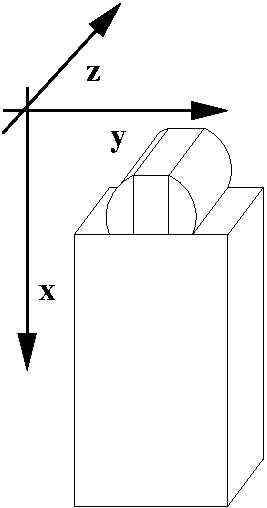
\includegraphics{images/axes}
\caption{Definition of axes in MMonCa}
\end{center}
\label{fig:axes}
\end{figure}

\begin{description}
\item [material=$<$procedure$>$] Specifies the name of a procedure where \MMonCa{} will obtain the material information. The procedure has three input arguments, x, y and z, and returns the name of a valid material.
\item [maxx=$<$X$>$] Maximum X size, in nanometers. (X is depth, see Fig.~\ref{fig:axes})
\item [maxy=$<$Y$>$] Maximum Y size, in nm. Y is width.
\item [maxz=$<$Z$>$] Maximum Z size, in nm.
\item [minx=$<$x$>$] Minimum x size.
\item [miny=$<$y$>$] Minimum y size.
\item [minz=$<$z$>$] Minimum z size.
\end{description}

Alternatively it is also possible to load a MeshParser grid file containing all the geometrical and material information. This file has explicitelly to include definitions and sizes of all the volumes involved in the simulation; i.e. underlying substrates, specific structures as well as the gas volumes used in CVD chambers, etc.

\begin{description}
\item [mesh=$<$filename$>$] Specifies the name of the MeshParser file. At this point, only .grd files are able to be loaded (no .bnd nor .dat).
\item [scale=$<$scale$>$] Scaling factor to be applied to the units used in the vertices definition inside the MeshParser file. Its value is 1000 by default for converting micrometers (common unit in microelectronics) to nanometers.
\end{description}

\subsection{Examples}
Example 1:
\begin{lstlisting}
proc material { x y z } {
        if { $x < 0 } { return "Gas" }
        return "Iron"
}
set sizeX  8
set sizeYZ 80
init minx=-2 miny=0 minz=0 maxx=$sizeX maxy=$sizeYZ maxz=$sizeYZ material=material
\end{lstlisting}

Example 2:
\begin{lstlisting}
init mesh=test_grid.grd scale=100
\end{lstlisting}
